\documentclass[border=10pt]{standalone}
\usepackage{tikz}
\usetikzlibrary{arrows.meta, shapes.geometric, positioning, calc}

\begin{document}
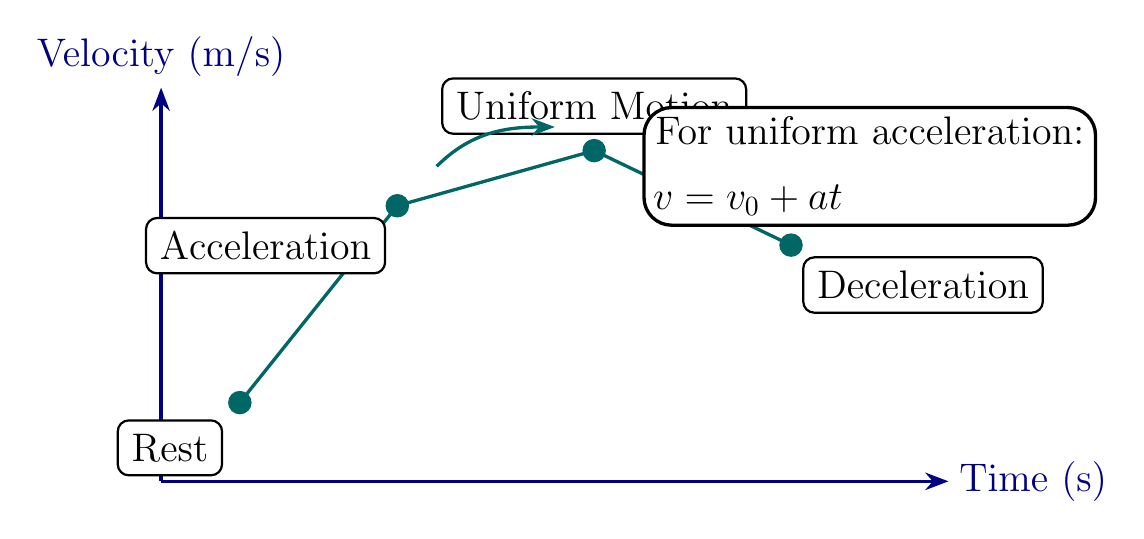
\begin{tikzpicture}[
    >=Stealth,
    node/.style={circle, fill=teal!80!black, inner sep=3pt},
    label/.style={rectangle, rounded corners, fill=white, draw=black, thick, inner sep=5pt, font=\Large},
    axis/.style={very thick, ->, blue!50!black}
]

% Axes
\draw[axis] (0,0) -- (10,0) node[right, font=\Large] {Time (s)};
\draw[axis] (0,0) -- (0,5) node[above, font=\Large] {Velocity (m/s)};

% Graph points
\coordinate (rest) at (1,1);
\coordinate (accel) at (3,3.5);
\coordinate (uniform) at (5.5,4.2);
\coordinate (decel) at (8,3);

% Graph line
\draw[very thick, teal!80!black] (rest) -- (accel) -- (uniform) -- (decel);

% Nodes
\node[node] at (rest) {};
\node[node] at (accel) {};
\node[node] at (uniform) {};
\node[node] at (decel) {};

% Labels
\node[label, below left=0.3cm of rest] {Rest};
\node[label, below left=0.2cm of accel] {Acceleration};
\node[label, above=0.2cm of uniform] {Uniform Motion};
\node[label, below right=0.2cm of decel] {Deceleration};

% Curved arrow from Acceleration to Uniform Motion
\draw[->, very thick, teal!80!black] ($(accel)+(0.5,0.5)$) to[out=45, in=180] ($(uniform)+(-0.5,0.3)$);

% Formula box
\node[rectangle, rounded corners=10pt, draw=black, very thick, fill=white, 
      text width=5.5cm, align=left, font=\Large] at (9,4) {
    \centering
    For uniform acceleration:\\[0.2cm]
    $v = v_0 + at$
};

\end{tikzpicture}
\end{document}